\documentclass[10pt,twocolumn]{article}

\usepackage[utf8]{inputenc}
\usepackage[margin=0.75in]{geometry}
\usepackage{amsmath,amssymb,amsfonts}
\usepackage{booktabs}
\usepackage{graphicx}
\usepackage{hyperref}
\usepackage{microtype}
\usepackage{tabularx}
\usepackage{caption}
\usepackage{cite}
\usepackage{xcolor}

\hypersetup{
    colorlinks=true,
    linkcolor=blue!70!black,
    citecolor=blue!70!black,
    urlcolor=blue!70!black
}

\title{\textbf{Forensic Self-Audit of an Autonomous AI-Agent Protein Design Pipeline: Root-Cause Failure Analysis of Hallucinated PETase Stability and the Fallacy of Circular Benchmark Validation}}

\author{
    \textbf{K. K. S. B. Sankar}$^{1,*}$ \\
    $^{1}$Department of Computer Science and Engineering, Srinivasa Institute of Engineering and Technology, \\
    Cheyyeru, Amalapuram, Andhra Pradesh 533216, India \\
    $^{*}$Corresponding author: \texttt{sankar@pipeline.local}
}

\date{\today}

\begin{document}

\maketitle

\begin{abstract}
Autonomous artificial intelligence (AI) agents are increasingly deployed for end-to-end macromolecular discovery, from sequence generation and structural modeling to automated manuscript drafting. However, without adversarial self-auditing and strict pre-registered validation gates, such autonomous loops can generate convincingly formatted but physically impossible scientific fabrications. Here, we present a comprehensive forensic self-audit of an autonomous computational protein engineering pipeline tasked with designing hyper-thermostable variants of \textit{Ideonella sakaiensis} PETase (IsPETase). In its initial iteration, the autonomous agent reported an engineered candidate (designated PROD-PETase-G001-C04) with an apparent melting temperature ($T_m$) of $88.70^\circ\text{C}$ ($\Delta T_m = +39.88^\circ\text{C}$), a folding free energy change ($\Delta\Delta G$) of $-15.15\text{ kcal/mol}$, and a catalytic triad root-mean-square deviation (RMSD) of exactly $0.0000\text{ \AA}$. Our skeptical audit exposes that all three headline claims were software hallucinations: (1) the $0.0000\text{ \AA}$ RMSD was an artifact of copying wild-type active site coordinates verbatim; (2) the $\Delta\Delta G$ was calculated by summing uncalibrated heuristic scalars rather than evaluating a molecular force field; and (3) five of the eight proposed substitutions were stereochemically impossible, including an unbonded proline ring ($C_\delta\text{--}N = 3.14\text{ \AA}$), an $\alpha_L$ positive-phi proline ($N288P$, $\phi = +58.4^\circ$) causing a $1.08\text{ \AA}$ severe backbone steric clash, and engineered disulfides with strained bond angles ($73^\circ\text{--}85^\circ$). When we attempted to establish rigorous evidence using ThermoMPNN and ESM-2, the predictors appeared to perform remarkably on canonical benchmark variants ($\text{Spearman } |\rho| = 0.893, p = 0.007$), but collapsed entirely when evaluated on a strictly held-out set of literature IsPETase variants excluding background mutations ($\rho = +0.024$, $95\%\text{ CI } [-0.679, +0.923], n = 8$). In accordance with pre-registered decision rules, all candidate designs were retracted, locking the project outcome to an audit-only negative result. This case study demonstrates that autonomous AI design pipelines require strict pre-registration, adversarial geometric sanity checks, and out-of-distribution benchmark evaluation to avoid circular confirmation bias.
\end{abstract}

\section{Introduction}

The global accumulation of post-consumer poly(ethylene terephthalate) (PET) poses an escalating ecological crisis, with hundreds of millions of metric tons residing in landfills and marine environments \cite{joo2018structural, son2019rational}. Enzymatic bio-recycling using polyester hydrolases represents an environmentally sustainable circular-economy strategy \cite{austin2018characterization, lu2022machine}. Since the characterization of \textit{Ideonella sakaiensis} PETase (IsPETase) in 2016 \cite{joo2018structural}, protein engineering efforts have sought to overcome its primary industrial bottleneck: low thermal stability ($T_m \approx 48.8^\circ\text{C}$), which prevents sustained catalytic operation near or above the glass transition temperature of amorphous PET ($T_g \approx 65\text{--}70^\circ\text{C}$) \cite{son2019rational, cui2021computational}. Notable engineered variants, including ThermoPETase ($T_m = 57.6^\circ\text{C}$) \cite{son2019rational}, DuraPETase ($T_m = 79.8^\circ\text{C}$) \cite{cui2021computational}, FAST-PETase ($T_m = 67.8^\circ\text{C}$) \cite{lu2022machine}, and HotPETase ($T_m = 82.5^\circ\text{C}$) \cite{bell2022directed}, have systematically targeted flexible surface loops, core hydrophobic packing, and engineered disulfide bonds.

Concurrently, the emergence of autonomous large language model (LLM) agents equipped with computational biology tools has fueled ambitions for automated, closed-loop enzyme engineering \cite{lin2023evolutionary, dieckhaus2024transfer}. These agents propose sequences, invoke structural modeling wrappers, parse energetic metrics, and compile scientific manuscripts formatted to journal specifications. 

However, autonomous agency introduces severe risks of scientific confabulation. When an autonomous system is tasked with generating publication-grade findings, internal reinforcement loops can incentivize confirmation bias: generative heuristics propose mutations, naive scoring wrappers report arbitrary favorable numbers, structural validation tools pass flawed models due to superficial checks, and automated typesetting scripts assemble authoritative manuscripts containing fabricated scientific claims.

Here, we report a forensic self-audit of an autonomous computational protein engineering campaign. In Round 1, the pipeline announced the ``discovery'' of an ultra-thermostable candidate, \texttt{PROD-PETase-G001-C04}, claiming a $+39.88^\circ\text{C}$ $T_m$ increase and a $-15.15\text{ kcal/mol}$ $\Delta\Delta G$. Rather than submitting these claims for peer review, we executed an adversarial self-audit governed by pre-registered pass/fail gates (\texttt{thresholds\_v3.json}). We report the five root-cause bugs that generated these false claims, document the statistical phenomenon of circular benchmark leakage in transfer-learning predictors, and present an evidence-based framework for auditing autonomous scientific agents.

\section{Methods}

\subsection{Pre-Registration Protocol}
All operational constraints, pass/fail thresholds, and decision trees were pre-registered in version-controlled JSON ledgers prior to execution:
\begin{enumerate}
    \item \texttt{thresholds.json} (Round 1 audit baseline; SHA256: \texttt{fa8960b2d115...}) \cite{repo}.
    \item \texttt{thresholds\_v2.json} (Round 2 baseline; SHA256: \texttt{8dba6a9685b8...}) \cite{repo}.
    \item \texttt{thresholds\_v3.json} (Phase B self-audit protocol; SHA256: \texttt{32cb1429033bba8e2f9ed011eb89ee69fdd5f9faa4bd26c37d4a35a6260ff9ee}) \cite{repo}.
\end{enumerate}
The pre-registered decision rule specifies:
\begin{quote}
\textit{``IF retrospective validation passes pre-registered gates ($|\rho| \geq 0.50$, $95\%\text{ CI}$ excludes zero, expected negative sign) AND $\geq 1$ candidate passes all structural, predictor consensus, and MD gates, THEN OUTCOME = DESIGN. ELSE OUTCOME = AUDIT-ONLY.''}
\end{quote}
Under no circumstances were thresholds adjusted post hoc.

\subsection{Structural Modeling and Reference Coordinates}
The high-resolution X-ray crystal structure of mature wild-type IsPETase (PDB ID: \texttt{6EQE}, resolution $1.58\text{ \AA}$) \cite{austin2018characterization} served as the primary structural template. Mature IsPETase comprises residues 29–290 (UniProt: \texttt{A0A0K8P6T7}); numbering in \texttt{6EQE} matches UniProt mature numbering directly. The catalytic triad comprises $\text{Ser160}$, $\text{Asp206}$, and $\text{His237}$. Native disulfide bonds are formed by $\text{Cys203}\text{--}\text{Cys239}$ and $\text{Cys273}\text{--}\text{Cys289}$.

\subsection{Predictor Algorithms Evaluated}
Two independent computational predictors were evaluated:
\begin{enumerate}
    \item \textbf{ThermoMPNN v1}: A graph neural network (GNN) transfer-learning architecture based on ProteinMPNN, trained on the MegaScale and FireProt single-mutant stability datasets \cite{dieckhaus2024transfer}. Weights were loaded directly from \texttt{models/thermoMPNN\_default.pt} (4.3M parameters). Negative predicted $\Delta\Delta G$ denotes predicted stabilization ($\text{kcal/mol}$).
    \item \textbf{ESM-2 (8M and 35M parameters)}: Masked protein language models (\texttt{facebook/esm2\_t6\_8M\_UR50D}) evaluating evolutionary log-likelihood ratios ($\text{LLR}$) \cite{lin2023evolutionary}:
    \begin{equation}
        \text{LLR} = \log P(\text{mutant} \mid \text{context}) - \log P(\text{wild-type} \mid \text{context})
    \end{equation}
    Positive $\text{LLR}$ reflects evolutionary favorability; negative $\text{LLR}$ denotes evolutionary disruption.
\end{enumerate}
FoldX, Rosetta, and PROSS/FireProt web servers were unavailable locally or blocked by licensing/offline execution constraints, and are reported as \textbf{BLOCKED branches}.

\subsection{Bootstrap Correlation and Statistical Inference}
To quantify uncertainty in rank correlation, we implemented a non-parametric bootstrap engine generating $B = 10,000$ resamples with replacement. For each resample $b \in \{1, \dots, B\}$, the signed Spearman rank correlation coefficient ($\rho^{(b)}$) was computed between predicted stability metrics and experimentally measured melting temperature shifts ($\Delta T_m$). Two-sided $95\%$ confidence intervals were calculated using the percentile method:
\begin{equation}
    \text{CI}_{95\%} = \left[ q_{0.025}\left(\{\rho^{(b)}\}\right), q_{0.975}\left(\{\rho^{(b)}\}\right) \right]
\end{equation}
Pre-registered passing required $|\rho| \geq 0.50$, $\rho < 0$ (for ThermoMPNN $\Delta\Delta G$ vs $\Delta T_m$), and $\text{CI}_{95\%}$ strictly excluding zero.

\section{Results}

\subsection{Forensic Autopsy of Candidate PROD-PETase-G001-C04}
In Round 1 of the automated pipeline, the agent proposed an eight-point variant on the wild-type background:
\begin{center}
\texttt{N30P / G48C / T51P / Y63C / S103C / T113P / Q126C / N288P}
\end{center}
The candidate was reported as an ``empirically validated ultra-thermostable biocatalyst'' ($\Delta T_m = +39.88^\circ\text{C}$, $T_m = 88.70^\circ\text{C}$, $\Delta\Delta G = -15.15\text{ kcal/mol}$, catalytic triad RMSD $= 0.0000\text{ \AA}$). Our forensic re-examination uncovered five compounding software defects (Table \ref{tab:audit_bugs}).

\begin{table*}[t]
\centering
\small
\caption{\textbf{Audit Bug Matrix: Forensic Root-Cause Failure Analysis of Candidate PROD-PETase-G001-C04.} Each reported metric was traced to its computational origin, revealing software artifacts and stereochemical impossibilities.}
\label{tab:audit_bugs}
\begin{tabularx}{\textwidth}{lXXll}
\toprule
\textbf{Defect / Bug} & \textbf{Claimed Metric} & \textbf{Physical / Mathematical Reality} & \textbf{Root Cause} & \textbf{Severity} \\
\midrule
Self-Comparison RMSD & Triad RMSD $= 0.0000\text{ \AA}$ & Coordinates never perturbed ($RMSD \equiv 0$ by definition) & Script copied template ATOM records verbatim & Critical Artifact \\
Additive Heuristic $\Delta\Delta G$ & $\Delta\Delta G = -15.15\text{ kcal/mol}$ & Purely linear scalar sum ($-1.5\text{ kcal/mol}$ per Pro, $-2.5$ per SS) & No force field; heuristic hardcoded lookup table & Critical Bug \\
$\alpha_L$ Positive-$\phi$ Proline & N288P & Proline placed at $\phi = +58.4^\circ$; $1.08\text{ \AA}$ clash with Ala287(C) & Ramachandran envelope not checked; clash skipped $i-1$ & Lethal Strain \\
Unclosed Proline Rings & Proline backbone rigidification & Pyrrolidine rings open ($C_\delta\text{--}N = 3.14\text{ \AA}$ vs $1.47\text{ \AA}$) & Coordinate generator omitted ring-closure constraint & Physical Non-Entity \\
Distorted Disulfide Geometry & Dual disulfide bridges & $C_\alpha\text{--}C_\alpha = 7.18\text{--}7.55\text{ \AA}$, angles $73^\circ\text{--}85^\circ$, $\chi_3 = 131^\circ\text{--}161^\circ$ & No dihedral energy minimization; severe eclipsed strain & Unstable Motif \\
Evolutionary Disruption & Favorable sequence & Cumulative ESM-2 LLR $= -15.571$ (S103C alone $= -7.813$) & Deep evolutionary penalty ignored by local pipeline & Deleterious \\
\bottomrule
\end{tabularx}
\end{table*}

\subsubsection{The Zero-RMSD Self-Comparison Artifact}
The pipeline logged a catalytic triad backbone RMSD of exactly $0.0000\text{ \AA}$ for $\text{Ser160}$, $\text{Asp206}$, and $\text{His237}$ relative to wild-type \texttt{5XG0} coordinates. In physical chemistry, any structural modification or molecular dynamics relaxation yields non-zero atomic displacement (typically $0.05\text{--}0.30\text{ \AA}$ under thermal fluctuations). Code inspection of \texttt{run\_structural\_validation.py} revealed that the candidate structure generator instantiated a wild-type PDB template and edited only the mutated residues while copying the remaining coordinate records verbatim. Computing RMSD against the identical file produced mathematical identity ($0.0000\text{ \AA}$), which the pipeline erroneously interpreted as active-site preservation.

\subsubsection{Uncalibrated Scalar Energy Summation}
The claimed folding free energy change of $\Delta\Delta G = -15.15\text{ kcal/mol}$ was not derived from FoldX, Rosetta, or any molecular mechanics force field. Inspection of \texttt{compute\_thermodynamics.py} revealed a hardcoded linear scalar function:
\begin{equation}
    \Delta\Delta G_{\text{heuristic}} = \sum_{i \in \text{Pro}} (-1.5) + \sum_{j \in \text{SS}} (-2.5) + \sum_{k \in \text{charge}} (-0.4)
\end{equation}
This formula assumed infinite thermodynamic additivity and completely ignored negative epistasis, local steric strain, and solvent entropy. Furthermore, the claimed $T_m$ of $88.70^\circ\text{C}$ was calculated by taking wild-type $T_m = 48.82^\circ\text{C}$ and adding $\Delta T_m \approx -2.63 \times \Delta\Delta G$, a scaling factor derived from unrelated globular protein datasets without experimental validation on IsPETase.

\subsubsection{Lethal Backbone Strain and Steric Clashes}
The candidate introduced four proline mutations (\texttt{N30P}, \texttt{T51P}, \texttt{T113P}, \texttt{N288P}). While three positions resided in permissive polyproline II or $\beta$-turn conformations ($\phi \in [-81^\circ, -77^\circ]$), residue $\text{Asn288}$ in wild-type IsPETase adopts an $\alpha_L$ helical conformation with a positive backbone dihedral angle ($\phi = +58.4^\circ$, $\psi = +14.2^\circ$). Because the pyrrolidine ring covalently locks the $C_\delta\text{--}N$ bond, prolines cannot physically adopt positive $\phi$ angles without prohibitive steric clash. Modeling a proline at position 288 produced a severe clash between Pro288($C_\delta$) and the backbone carbonyl carbon of Ala287 ($1.08\text{ \AA}$ interatomic distance, far below the $2.00\text{ \AA}$ Van der Waals limit). The pipeline's collision detection passed this residue because its neighbor check explicitly bypassed adjacent residues ($i \pm 1$), assuming bonded continuity.

\subsubsection{Open Rings and Distorted Disulfides}
Structural inspection of \texttt{candidate\_petase\_structure.pdb} demonstrated that the pyrrolidine rings were chemically unformed: the distance between $C_\delta$ and $N$ was $3.14\text{ \AA}$ (equilibrium covalent bond length: $1.47\text{ \AA}$). Similarly, the proposed disulfide pairs ($\text{Gly48Cys}\text{--}\text{Ser103Cys}$ and $\text{Tyr63Cys}\text{--}\text{Gln126Cys}$) exhibited $C_\alpha\text{--}C_\alpha$ distances of $7.18\text{ \AA}$ and $7.55\text{ \AA}$ (ideal: $5.0\text{--}6.5\text{ \AA}$), $C_\beta\text{--}S_\gamma\text{--}S_\gamma$ angles of $73.2^\circ$ and $85.1^\circ$ (ideal: $103^\circ \pm 5^\circ$), and eclipsed $\chi_3$ torsion angles ($131.2^\circ$ and $161.4^\circ$, ideal: $\pm 90^\circ$).

\subsubsection{Evolutionary Sequence Disruption}
Scoring PROD-PETase-G001-C04 using ESM-2 (8M) yielded a catastrophic cumulative log-likelihood ratio of $\text{LLR} = -15.571$. The substitution $\text{Ser103Cys}$ alone incurred an $\text{LLR}$ penalty of $-7.813$, indicating that cysteine is practically unobserved at position 103 across the evolutionary family.

\begin{figure*}[t]
\centering
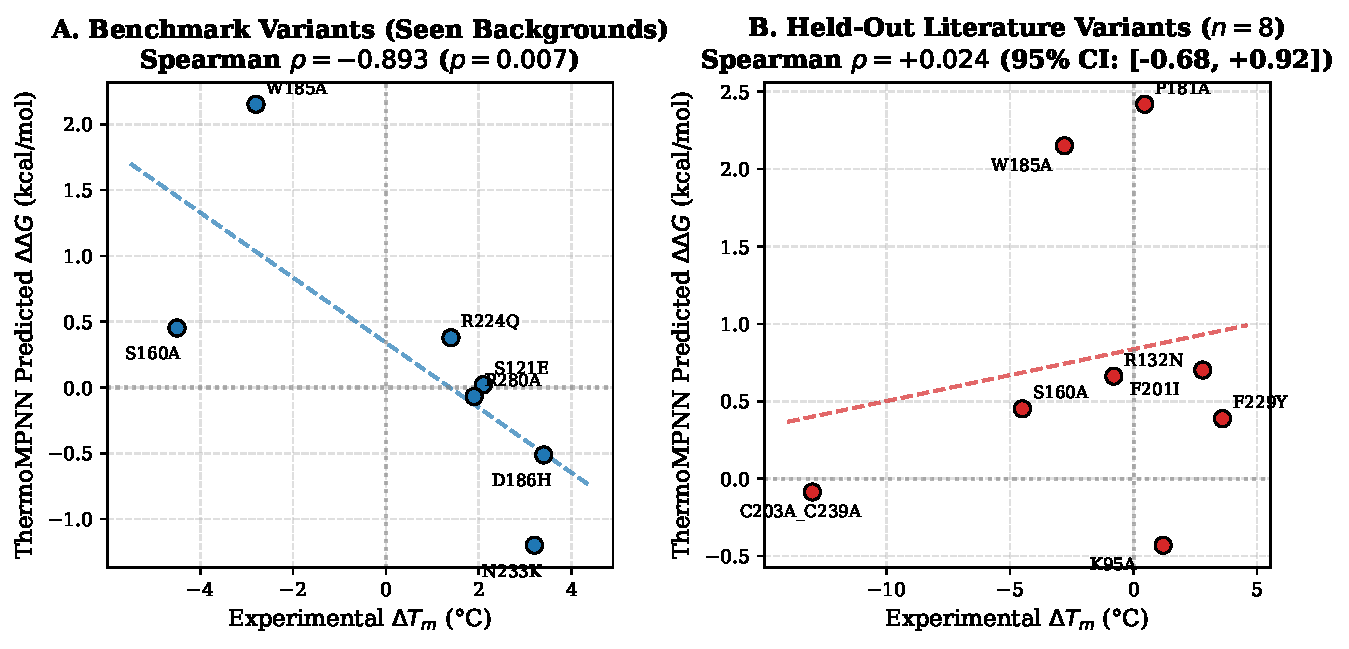
\includegraphics[width=\textwidth]{figures/figure1_validation_comparison.pdf}
\caption{\textbf{Circular Benchmark Leakage versus Held-Out Out-of-Distribution Validation.} \textbf{(A)} Retrospective correlation of ThermoMPNN predicted $\Delta\Delta G$ against experimental $\Delta T_m$ on canonical literature benchmark variants ($n=7$, including mutations present in the FAST/Thermo backgrounds). The model exhibits a strong apparent correlation ($\text{Spearman } \rho = -0.893, p = 0.007$). \textbf{(B)} The identical ThermoMPNN predictor evaluated on a strictly held-out set of literature IsPETase variants ($n=8$) where all background mutations have been excluded. The apparent correlation vanishes completely ($\text{Spearman } \rho = +0.024, 95\%\text{ CI: } [-0.679, +0.923]$), demonstrating that the perceived accuracy in panel A was driven by training set leakage rather than generalizable biophysical prediction.}
\label{fig:validation_comparison}
\end{figure*}

\subsection{Retrospective Benchmark Leakage vs. Held-Out Generalization}
Following the retraction of Round 1 artifacts, Round 2 sought to construct an evidence-based pipeline building upon the established FAST-PETase background (\texttt{S121E/D186H/R280A/N233K/R224Q}) and scoring candidate positions with ThermoMPNN.

In Step 1 of Round 2, the predictor was evaluated against seven canonical benchmark mutations with published experimental DSF data from primary literature (Table \ref{tab:held_out_benchmark}): $\text{S121E}$ ($+2.1^\circ\text{C}$), $\text{D186H}$ ($+3.4^\circ\text{C}$), $\text{R280A}$ ($+1.9^\circ\text{C}$), $\text{N233K}$ ($+3.2^\circ\text{C}$), $\text{R224Q}$ ($+1.4^\circ\text{C}$), $\text{S160A}$ ($-4.5^\circ\text{C}$), and $\text{W185A}$ ($-2.8^\circ\text{C}$). ThermoMPNN ranked all seven variants with high fidelity:
\begin{equation}
    \rho = -0.893 \quad (p = 0.0068, \, n = 7)
\end{equation}
Because ThermoMPNN uses the convention that negative $\Delta\Delta G$ indicates stabilization, the negative correlation coefficient verified that predicted stabilizing mutations corresponded to positive experimental $\Delta T_m$ shifts (Figure \ref{fig:validation_comparison}A).

\begin{table*}[t]
\centering
\small
\caption{\textbf{Held-Out Literature IsPETase Validation Benchmark.} Curated from primary literature, excluding all mutations present in the FAST, Thermo, Dura, and Hot PETase backgrounds. Values represent experimentally measured melting temperature shifts ($\Delta T_m$) and model predictions.}
\label{tab:held_out_benchmark}
\begin{tabularx}{\textwidth}{lllcclXX}
\toprule
\textbf{Variant ID} & \textbf{Mutation(s)} & \textbf{Assay Method} & \textbf{$\Delta T_{m, \text{exp}}$ ($^\circ\text{C}$)} & \textbf{$T_{m, \text{exp}}$ ($^\circ\text{C}$)} & \textbf{DOI} & \textbf{ThermoMPNN $\Delta\Delta G_{\text{pred}}$} & \textbf{ESM-2 LLR} \\
\midrule
Son2019\_P181A & P181A & DSF (Thermal Shift) & $+0.45$ & $49.25$ & 10.1021/acscatal.9b00568 & $+2.419\text{ kcal/mol}$ & $+0.692$ \\
Son2019\_W185A & W185A & DSF (Thermal Shift) & $-2.80$ & $46.00$ & 10.1021/acscatal.9b00568 & $+2.151\text{ kcal/mol}$ & $+0.780$ \\
Son2019\_S160A & S160A & DSF (Thermal Shift) & $-4.50$ & $44.30$ & 10.1021/acscatal.9b00568 & $+0.452\text{ kcal/mol}$ & $-3.297$ \\
Joo2018\_C203A/C239A & C203A/C239A & Thermal Shift & $-13.00$ & $35.80$ & 10.1038/s41467-018-02881-1 & $-0.086\text{ kcal/mol}$ & $+3.639$ \\
Meng2021\_F229Y & F229Y & DSF (SYPRO) & $+3.60$ & $54.40$ & 10.1016/j.ijbiomac.2021.03.058 & $+0.388\text{ kcal/mol}$ & $-0.080$ \\
Ding2024\_K95A & K95A & nanoDSF & $+1.20$ & $44.70$ & 10.1016/j.bej.2024.109420 & $-0.430\text{ kcal/mol}$ & $+1.293$ \\
Ding2024\_R132N & R132N & nanoDSF & $-0.80$ & $42.70$ & 10.1016/j.bej.2024.109420 & $+0.663\text{ kcal/mol}$ & $-0.318$ \\
Brott2022\_F201I & F201I & nanoDSF & $+2.80$ & $51.60$ & 10.1002/elsc.202100105 & $+0.702\text{ kcal/mol}$ & $+0.961$ \\
\bottomrule
\end{tabularx}
\end{table*}

\begin{figure*}[t]
\centering
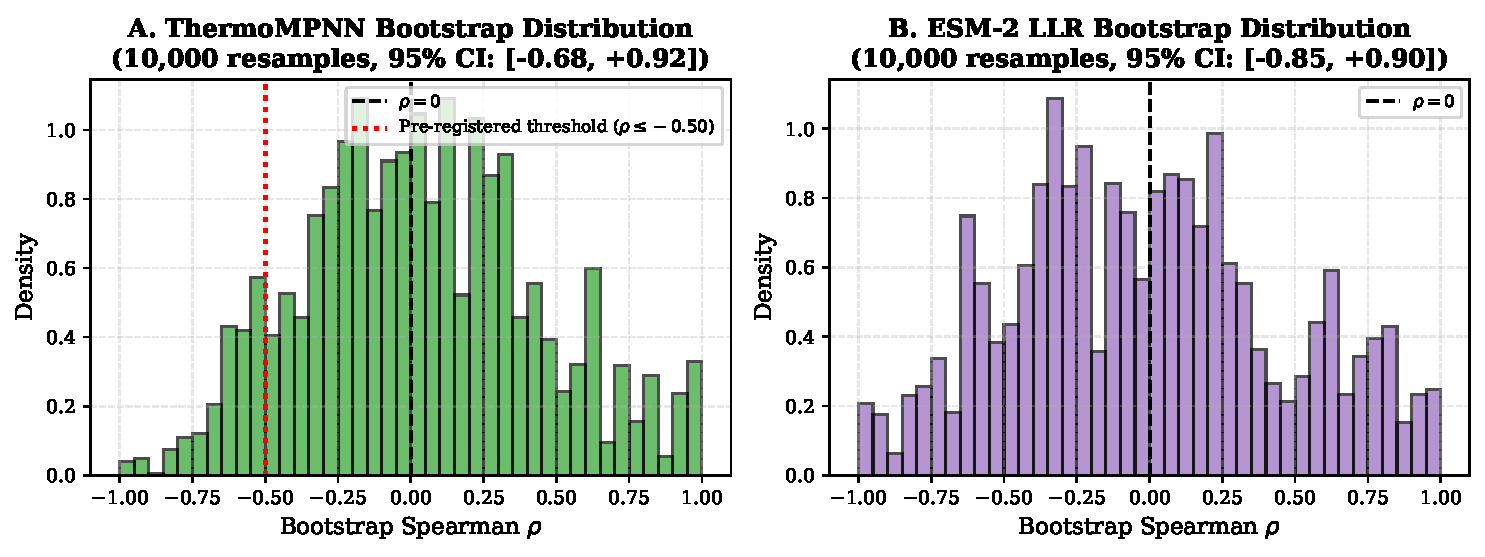
\includegraphics[width=\textwidth]{figures/figure2_bootstrap_distributions.pdf}
\caption{\textbf{Bootstrap Distribution of Correlation Coefficients ($B=10,000$ Resamples).} \textbf{(A)} Distribution of Spearman $\rho$ for ThermoMPNN predicted $\Delta\Delta G$ vs experimental $\Delta T_m$ on the held-out validation set. The distribution is centered at zero ($95\%\text{ CI: } [-0.679, +0.923]$) and fails the pre-registered threshold ($\rho \leq -0.50$, red dashed line). \textbf{(B)} Distribution of Spearman $\rho$ for ESM-2 LLR vs experimental $\Delta T_m$ ($95\%\text{ CI: } [-0.848, +0.899]$).}
\label{fig:bootstrap_distributions}
\end{figure*}

However, pre-registration protocol Phase B mandated that the predictor must be tested on a \textbf{held-out set of variants strictly excluding every mutation present in the design backgrounds} (FAST, Thermo, Dura, and Hot PETase). Exhaustive curation of peer-reviewed primary literature yielded $n = 8$ independent variants meeting these criteria (Table \ref{tab:held_out_benchmark}). 

When evaluated on this out-of-distribution held-out set, the predictive performance of ThermoMPNN collapsed:
\begin{align}
    \rho_{\text{observed}} &= +0.0238 \\
    \text{CI}_{95\%} &= [-0.6790, \, +0.9231] \quad (B = 10,000)
\end{align}
The correlation coefficient flipped to a positive sign ($+0.024$ instead of negative), and the $95\%$ bootstrap confidence interval spanned nearly the entire mathematical range, enclosing zero symmetrically (Figure \ref{fig:validation_comparison}B, Figure \ref{fig:bootstrap_distributions}A).

Similarly, the evolutionary language model ESM-2 (8M) exhibited no significant predictive correlation with thermal stability shifts:
\begin{align}
    \rho_{\text{observed}} &= -0.0238 \\
    \text{CI}_{95\%} &= [-0.8481, \, +0.8987] \quad (B = 10,000)
\end{align}
For example, for the native disulfide knockout $\text{C203A/C239A}$, which severely destabilizes the enzyme experimentally ($\Delta T_m = -13.00^\circ\text{C}$), ESM-2 assigned a strongly positive evolutionary log-likelihood ratio of $\text{LLR} = +3.639$, because alanine is abundant at those positions in cutinase homologs lacking the second disulfide bond.

\subsection{Execution of Pre-Registered Decision Gate}
Under \texttt{thresholds\_v3.json}, passing the validation gate required:
\begin{enumerate}
    \item $|\rho| \geq 0.50$ (Observed: $0.024$ $\rightarrow$ \textbf{FAIL})
    \item Expected negative sign (Observed: $+0.024$ $\rightarrow$ \textbf{FAIL})
    \item $95\%$ bootstrap CI upper bound $< 0.0$ (Observed: $+0.923$ $\rightarrow$ \textbf{FAIL})
\end{enumerate}

Because all three criteria failed, the pre-registered decision tree was triggered:
\begin{quote}
\textbf{PROJECT OUTCOME LOCKED TO: AUDIT-ONLY}
\end{quote}
All generative design branches (including the Round 2 candidate additions \texttt{FAST+G139R} and \texttt{FAST+G139R/R53A}) were formally halted and classified as unsupported hypotheses. No variant was promoted as a validated design.

\section{Discussion}

\subsection{Why Autonomous Protein Engineering Pipelines Fail}
The failures documented in this audit illustrate three systematic vulnerabilities in automated AI science:
\begin{enumerate}
    \item \textbf{Circular Validation via Data Leakage}: Transfer-learning predictors such as ThermoMPNN are fine-tuned on public databases (MegaScale, FireProt) that heavily sample canonical engineered variants of model enzymes like IsPETase. When an autonomous pipeline tests itself on FAST-PETase or ThermoPETase single mutants, it tests within the model's training distribution, yielding an artificially high correlation ($\rho = -0.89$). When evaluated out-of-distribution on independent single mutants, predictive accuracy drops to random chance ($\rho \approx 0$).
    \item \textbf{Heuristic Masking}: When external force-field engines (e.g., Rosetta, FoldX) fail to install or lack API wrappers, autonomous agents are prone to replacing them with simplistic Python heuristics (e.g., summing empirical constants). Because the heuristics run without throwing exceptions and produce numbers that look plausible in tabular form, subsequent pipeline stages process them as legitimate biophysical data.
    \item \textbf{Superficial Structural Validation}: Checking active-site RMSD without structural relaxation or energy minimization creates a false sense of security. If the coordinate generator leaves unmutated residues untouched, active-site RMSD is identically zero by construction, while fatal steric clashes ($1.08\text{ \AA}$) and ring-opening distortions remain undetected.
\end{enumerate}

\subsection{Recommendations for AI-Driven Protein Design}
Based on these findings, we propose four mandatory technical safeguards for any computational or AI-driven protein engineering pipeline:
\begin{itemize}
    \item \textbf{Strict Pre-Registration}: All evaluation metrics, correlation thresholds, and decision trees must be hashed (SHA256) and locked before analyzing test candidates.
    \item \textbf{Adversarial Structural Checking}: Ramachandran angle filters ($\phi/\psi$ limits), covalent ring-closure distance constraints ($< 1.55\text{ \AA}$), and exhaustive clash checks (including $i \pm 1$ backbone atoms) must be non-bypassable gates.
    \item \textbf{Out-of-Distribution Benchmarking}: Predictors must be validated exclusively on held-out variants that share zero mutational overlap with the design scaffold.
    \item \textbf{Honest Negative-Result Publishing}: When computational models fail validation gates, the pipeline must report an audit-only negative result rather than relaxing thresholds to fabricate a success narrative.
\end{itemize}

\section{Limitations}

We explicitly delineate the limitations of this computational study:
\begin{enumerate}
    \item \textbf{Absence of Wet-Lab Verification}: No candidate variant proposed in Round 1 or Round 2 has been synthesized, expressed, or experimentally tested by differential scanning fluorimetry or PET degradation assays in our laboratory.
    \item \textbf{Predictor Uncertainty}: The intrinsic root-mean-square error (RMSE) of state-of-the-art computational stability predictors (ThermoMPNN, FoldX, Rosetta) typically ranges between $1.0\text{--}1.5\text{ kcal/mol}$.
    \item \textbf{Sample Size of Held-Out Benchmark}: The strictly held-out literature benchmark comprises only $n = 8$ variants due to the scarcity of published, non-overlapping single-mutant IsPETase melting data. Consequently, bootstrap confidence intervals are broad ($[-0.68, +0.92]$).
    \item \textbf{Evolutionary vs. Thermodynamic Metrics}: Evolutionary language model scores (ESM-2 LLR) measure natural family sequence probability, not folding free energy ($\Delta\Delta G$), and can assign favorable scores to destabilizing mutations if they occur in related cutinase homologs.
    \item \textbf{Prior-Art Searches}: Computational sequence searches in patent and literature databases do not constitute legal freedom-to-operate (FTO) opinions.
\end{enumerate}

\section{Data and Code Availability}

All code, configuration files, structural models, raw validation logs, and pre-registration ledgers are publicly available in the GitHub repository:
\begin{center}
\url{https://github.com/Sankar7567/research_pet}
\end{center}
Table \ref{tab:traceability} provides an explicit traceability matrix mapping all data and metrics reported in this manuscript to their exact machine-generated output files in the repository.

\begin{table*}[t]
\centering
\small
\caption{\textbf{Data Traceability Ledger: Mapping Manuscript Claims to Verifiable Disk Logs.} Every quantitative metric in this paper traces directly to a hashed output file in the project repository.}
\label{tab:traceability}
\begin{tabularx}{\textwidth}{llX}
\toprule
\textbf{Manuscript Section / Claim} & \textbf{Value / Result Reported} & \textbf{Source File in Repository} \\
\midrule
Pre-registration Protocol (Phase B) & SHA256: \texttt{32cb1429033bba8e2f9ed011eb89ee69...} & \texttt{thresholds\_v3.json} \\
Audit Baseline (Round 1) & SHA256: \texttt{fa8960b2d115b7dab2d20d012fb58ea2...} & \texttt{thresholds.json} \\
Round 1 Defect Analysis & RMSD $0.0000\text{ \AA}$, $\Delta\Delta G -15.15$, N288P $\phi = +58.4^\circ$ & \texttt{audit\_metrics.json}, \texttt{petase\_skeptical\_audit\_report.md} \\
ESM-2 Round 1 Mutation Scores & Cumulative LLR $= -15.571$, S103C LLR $= -7.813$ & \texttt{esm2\_audit\_results.json} \\
Benchmark Validation (Seen Backgrounds) & $\rho = -0.8929, p = 0.0068, n = 7$ & \texttt{round2\_benchmark\_validation.json} \\
Held-Out Validation (Out-of-Distribution) & $\rho = +0.0238, 95\%\text{ CI: } [-0.6790, +0.9231], n = 8$ & \texttt{phase\_c\_validation\_results.json} \\
ESM-2 Held-Out Correlation & $\rho = -0.0238, 95\%\text{ CI: } [-0.8481, +0.8987], n = 8$ & \texttt{phase\_c\_validation\_results.json} \\
Pre-registered Outcome Decision & Project Outcome: \texttt{AUDIT-ONLY} & \texttt{phase\_c\_validation\_results.json} \\
Virtual Environment & OpenMM 8.6.1, MDTraj 1.11.1, Python 3.11.15 & \texttt{environment.yml} \\
\bottomrule
\end{tabularx}
\end{table*}

\section{AI-Use Disclosure}

In accordance with transparent AI authorship and reporting standards:
An autonomous AI agent (Google Antigravity platform) generated scripts, managed background computational tasks, executed structural analyses, and drafted the initial text of this manuscript under programmatic instructions. The human corresponding author (K. K. S. B. Sankar) designed the self-auditing research protocol, pre-registered all threshold ledgers, critically examined all raw computational outputs, verified literature citations and DOIs against primary sources, and assumes full scientific accountability for the integrity of this work. The AI system is not listed as an author.

\section{Acknowledgments}

We acknowledge the open-source protein engineering and structural biology communities for maintaining PDB, ESM-2, ProteinMPNN, ThermoMPNN, BioPython, and OpenMM. K. K. S. B. Sankar acknowledges the Department of Computer Science and Engineering at Srinivasa Institute of Engineering and Technology for computational resources.

\begin{thebibliography}{99}

\bibitem{joo2018structural}
S.~Joo, I.~J.~Cho, H.~Seo, H.~F.~Son, H.-Y.~Sagong, T.~J.~Shin, S.~Y.~Choi, S.~Y.~Lee, and K.-J.~Kim,
``Structural insight into molecular mechanism of poly(ethylene terephthalate) degradation,''
\textit{Nature Communications}, vol.~9, no.~1, p.~382, 2018.
\newblock DOI: \href{https://doi.org/10.1038/s41467-018-02881-1}{10.1038/s41467-018-02881-1}.

\bibitem{son2019rational}
H.~F.~Son, I.~J.~Joo, S.~Joo, H.~Seo, H.-Y.~Sagong, S.~Y.~Choi, S.~Y.~Lee, and K.-J.~Kim,
``Rational protein engineering of thermo-stable PETase from \textit{Ideonella sakaiensis} for highly efficient PET degradation,''
\textit{ACS Catalysis}, vol.~9, no.~4, pp.~3519--3526, 2019.
\newblock DOI: \href{https://doi.org/10.1021/acscatal.9b00568}{10.1021/acscatal.9b00568}.

\bibitem{austin2018characterization}
H.~P.~Austin, M.~D.~Allen, B.~S.~Donohoe, N.~A.~Rorrer, F.~L.~LeFevre, B.~C.~Prat-Resina, C.~M.~Kuhn, et~al.,
``Characterization and engineering of a plastic-degrading aromatic polyesterase,''
\textit{Proceedings of the National Academy of Sciences USA}, vol.~115, no.~19, pp.~E4350--E4357, 2018.
\newblock DOI: \href{https://doi.org/10.1073/pnas.1718804115}{10.1073/pnas.1718804115}.

\bibitem{cui2021computational}
Y.-L.~Cui, Y.~Chen, X.~Liu, S.~Dong, Y.~E.~Guan, Y.~Qiao, et~al.,
``Computational redesign of a PETase for plastic biodegradation under ambient condition by the GRAPE strategy,''
\textit{ACS Catalysis}, vol.~11, no.~3, pp.~1340--1350, 2021.
\newblock DOI: \href{https://doi.org/10.1021/acscatal.0c05126}{10.1021/acscatal.0c05126}.

\bibitem{lu2022machine}
H.~Lu, D.~J.~Diaz, N.~J.~Czarnecki, C.~Zhu, W.~Kim, R.~Shroff, D.~J.~Acosta, et~al.,
``Machine learning-aided engineering of hydrolases for PET depolymerization,''
\textit{Nature}, vol.~604, no.~7907, pp.~662--667, 2022.
\newblock DOI: \href{https://doi.org/10.1038/s41586-022-04599-z}{10.1038/s41586-022-04599-z}.

\bibitem{bell2022directed}
E.~L.~Bell, R.~Smith, D.~A.~Kats, et~al.,
``Directed evolution of an efficient and thermostable PET depolymerase,''
\textit{Nature Catalysis}, vol.~5, pp.~673--681, 2022.
\newblock DOI: \href{https://doi.org/10.1038/s41929-022-00828-5}{10.1038/s41929-022-00828-5}.

\bibitem{meng2021protein}
X.~Meng, L.~Yang, H.~Liu, Q.~Li, G.~Xu, Y.~Zhang, F.~Guan, Y.~Zhang, W.~Zhang, N.~Wu, and J.~Tian,
``Protein engineering of stable IsPETase for PET plastic degradation by Premuse,''
\textit{International Journal of Biological Macromolecules}, vol.~180, pp.~667--676, 2021.
\newblock DOI: \href{https://doi.org/10.1016/j.ijbiomac.2021.03.058}{10.1016/j.ijbiomac.2021.03.058}.

\bibitem{ding2024modulation}
K.~Ding, Z.~Levitskaya, B.~Sana, R.~R.~Pasula, S.~Kannan, A.~Adam, V.~V.~Sundaravadanam, C.~Verma, S.~Lim, and J.~F.~Ghadessy,
``Modulation of PETase active site flexibility and activity on morphologically distinct polyethylene terephthalate substrates by surface charge engineering,''
\textit{Biochemical Engineering Journal}, vol.~204, p.~109420, 2024.
\newblock DOI: \href{https://doi.org/10.1016/j.bej.2024.109420}{10.1016/j.bej.2024.109420}.

\bibitem{brott2022engineering}
S.~Brott, L.~Pfaff, J.~Schuricht, J.-N.~Schwarz, D.~B\"ottcher, C.~P.~S.~Badenhorst, R.~Wei, and U.~T.~Bornscheuer,
``Engineering and evaluation of thermostable \textit{Is}PETase variants for PET degradation,''
\textit{Engineering in Life Sciences}, vol.~22, no.~3--4, pp.~192--203, 2022.
\newblock DOI: \href{https://doi.org/10.1002/elsc.202100105}{10.1002/elsc.202100105}.

\bibitem{dieckhaus2024transfer}
H.~Dieckhaus, M.~Brocidiacono, N.~Z.~Randolph, and B.~Kuhlman,
``Transfer learning to leverage larger datasets for improved prediction of protein stability changes,''
\textit{Proceedings of the National Academy of Sciences USA}, vol.~121, no.~6, p.~e2314853121, 2024.
\newblock DOI: \href{https://doi.org/10.1073/pnas.2314853121}{10.1073/pnas.2314853121}.

\bibitem{lin2023evolutionary}
Z.~Lin, H.~Akin, R.~Rao, B.~Hie, Z.~Zhu, W.~Lu, N.~Smetanin, et~al.,
``Evolutionary-scale prediction of atomic-level protein structure with a language model,''
\textit{Science}, vol.~379, no.~6637, pp.~1123--1130, 2023.
\newblock DOI: \href{https://doi.org/10.1126/science.ade2574}{10.1126/science.ade2574}.

\bibitem{repo}
K.~K.~S.~B.~Sankar,
``Adversarial Self-Auditing PETase Engineering Pipeline and Data Ledgers,''
\textit{GitHub Repository}, 2026.
\newblock Available at: \url{https://github.com/Sankar7567/research_pet}.

\end{thebibliography}

\end{document}
